% Template for APA submission with R Markdown

% Stuff changed from PLOS Template
\documentclass[a4paper,man,apacite,floatsintext]{apa6}
\usepackage{apacite}

% amsmath package, useful for mathematical formulas
\usepackage{amsmath}
% amssymb package, useful for mathematical symbols
\usepackage{amssymb}

% hyperref package, useful for hyperlinks
\usepackage{hyperref}

% graphicx package, useful for including eps and pdf graphics
% include graphics with the command \includegraphics
\usepackage{graphicx}

% Sweave(-like)
\usepackage{fancyvrb}
\DefineVerbatimEnvironment{Sinput}{Verbatim}{fontshape=sl}
\DefineVerbatimEnvironment{Soutput}{Verbatim}{}
\DefineVerbatimEnvironment{Scode}{Verbatim}{fontshape=sl}
\newenvironment{Schunk}{}{}
\DefineVerbatimEnvironment{Code}{Verbatim}{}
\DefineVerbatimEnvironment{CodeInput}{Verbatim}{fontshape=sl}
\DefineVerbatimEnvironment{CodeOutput}{Verbatim}{}
\newenvironment{CodeChunk}{}{}

% cite package, to clean up citations in the main text. Do not remove.
\usepackage{cite}

\usepackage{color}

% Use doublespacing - comment out for single spacing
%\usepackage{setspace}
%\doublespacing


% Text layout
\topmargin 0.0cm
\oddsidemargin 0.5cm
\evensidemargin 0.5cm
\textwidth 16cm
\textheight 21cm

% Bold the 'Figure #' in the caption and separate it with a period
% Captions will be left justified
\usepackage[labelfont=bf,labelsep=period,justification=raggedright]{caption}


% Remove brackets from numbering in List of References
\makeatletter
\renewcommand{\@biblabel}[1]{\quad#1.}
\makeatother


% Leave date blank
\date{}

%\pagestyle{myheadings}
%% ** EDIT HERE **


%% ** EDIT HERE **
%% PLEASE INCLUDE ALL MACROS BELOW

%% END MACROS SECTION


% ALL OF THE TITLE PAGE INFORMATION IS SPECIFIED IN THE YAML
\title{\textbf{Children's social referencing reflects sensitivity to graded uncertainty}}
\shorttitle{}

\author{Emily Hembacher}

\affiliation{Department of Psychology, Stanford University}

\authornote{}
\abstract{This study examined a spontaneous information gathering behavior --
social referencing -- and its relation to epistemic uncertainty during
early childhood. Children ages 2-5 (\emph{n}=160) identified the
referents of familiar and novel labels. Referential ambiguity was
manipulated through the number of objects present and their familiarity
(Experiments 1 and 2), and the availability of referential gaze
(Experiment 2). In both experiments, children visually referenced the
experimenter more often while responding when the referent was
ambiguous. In Experiment 2, children also referenced more when there was
a novel referent and familiar distracter (and the referent could thus be
inferred), but only when referential gaze was unavailable. These results
suggest that children seek disambiguating social information on the
basis of graded uncertainty.}
\keywords{social referencing; help seeking; word learning; uncertainty.}

\begin{document}
\maketitle

Preschoolers quickly learn new concepts, rules, and language. They also
actively explore (Schulz \& Bonawitz, 2007) and ask questions
(Chouinard, Harris, \& Maratsos, 2007) in ways that seem targeted to
maximize learning. These behaviors appear to require children to monitor
epistemic states of ignorance and uncertainty, but young children have
generally been credited with limited ability to monitor mental states
(Sodian, Thoermer, Kristen, \& Perst, 2012). This presents a puzzle --
how do children acquire disambiguating information if they are not able
to monitor uncertainty? To better understand how young children actively
construct meaning from their environment, more evidence is needed about
the relation between epistemic uncertainty and information seeking in
early childhood. Do young children monitor uncertainty and engage in
active learning behaviors based on this monitoring, or is early learning
better characterized as a process of integrating information that is
generated externally, for example, by social partners who act as
teachers (Csibra \& Gergely, 2006)?

The literature on metacognitive development has typically attributed
limited capacities to young children. This attribution derives from a
few studies showing that young children cannot introspect on their
thoughts, and has also been assumed based on metacognitive failures in
older children. Lockl \& Schneider (2004) -- incentives and
instruction-- kids still fail at regulating study time.

Early research on metacognitive development suggested that young
children have limited capacities to reflect on their own thoughts or
knowledge. For example, In another study, 5-year-olds were found to have
limited awareness of their own ongoing thoughts (J. H. Flavell, Green,
Flavell, Harris, \& Astington, 1995). Often, researchers have declined
to investigate early metacognition altogether due to methodological
limitations, since most research in the metacognitive framework relies
on explicit verbal reports, which are inappropriate for young children.

However, these and other studies tended to rely on children's explicit
verbal reports about their mental operations, often in a free-response
format, which might underestimate children's ability to track epistemic
states.

More recently, researchers have begun to investigate children's
uncertainty monitoring using tasks that do not require a verbal response
from children. In one study, 3- to 5-year-olds completed perceptual
discrimination and lexical identification tasks and reported on their
certainty in their choices using a pictorial confidence scale (Lyons \&
Ghetti, 2011). Preschoolers reported being less confident when they
responded incorrectly, suggesting that they were aware of their
likelihood of accuracy based on their epistemic states. In another
study, 3.5-year-olds completed a memory task in which they could opt out
of responding to individual trials (Balcomb \& Gerken, 2008). Children
performed worse on trials they had opted out of when they were forced to
answer them later on, suggesting that children used the opt-out option
strategically to avoid answering when they were uncertain about their
responses. On the other hand, Hembacher and Ghetti (2014) found that
3-year-olds reported being equally confident for correct and incorrect
responses in a memory task using a pictorial confidence scale, while 4-
and 5-year-olds were less confident when incorrect, suggesting that
there are limits to 3-year-olds abilities to monitor uncertainty, and
that some cognitive states may be more easily reflected on by young
children than others. In sum, preschool-aged children demonstrate an
emerging awareness of epistemic uncertainty in laboratory tasks that do
not require a verbal or open-ended response. However, even the
competencies reported in these studies may underestimate children's
ability to track epistemic uncertainty and act on it.

In the following sections, we first outline an emerging body of research
that suggests that children actively gather data to support learning
from a young age, in a way that reflects sensitivity to epistemic
uncertainty. We then summarize previous work on children's ability to
selectively gather social information from credible sources and under
conditions of epistemic uncertainty.

\subsection{Active Learning in Early
Childhood}\label{active-learning-in-early-childhood}

Active learning refers broadly to learning behaviors and materials that
are initiated by the learner themself, rather than generated by a
teacher (refs). First, there are studies that take inspiration from
comparative metacognition research and ask whether children's
spontaneous information-seeking behaviors track uncertainty. For
example, Call and Carpenter (2001) had 2-year-olds choose between
several tubes to find a hidden sticker. They found that the toddlers
were more likely to peek inside a tube before choosing when they had not
seen the baiting of the tubes compared to when they had, suggesting they
were aware of their knowledge or ignorance and selectively sought
confirmatory evidence before committing to a response when they did not
know a sticker's location. In another study, Goupil, Romand-Monnier, and
Kouider (2016) trained 20-month-olds to look at their parents if they
needed help with a memory task in which they had to locate a hidden toy.
Toddlers were more likely to seek help when they were completely
ignorant of the toy's location, and when the task was more difficult
because the delay between hiding and test was longer.

Others have focused on children's spontaneous exploration of objects
under different epistemic conditions. Stahl \& Feigenson (2015) found
that 11-month-old infants were more likely to explore objects that had
violated physical expectations (e.g., a toy car that appeared to hover
in midair) than those that had made similar trajectories without
appearing to violate physics (e.g., a toy that moved along a platform).
Intriguingly, infants were more likely to explore the objects in ways
that were suited to testing the physical property they had seen violated
(e.g., picking up and dropping the car that had hovered in midair;
banging a toy that had appeared to move through a solid wall). These
results suggest that infants selectively explore objects to disambiguate
causal properties that have been rendered uncertain by a surprising
event.

There is also evidence that young children selectively explore when
evidence is confounded (i.e., when existing evidence supports multiple
causal hypotheses). For example, Schulz \& Bonawitz (2007) found that
preschoolers spent more time playing with a toy when they witnessed
confounded evidence about its causal structure. Children who experienced
a demonstration of a toy in which two levers were simultaneously
depressed and caused two simultaneous events (a toy duck and puppet
popping up) spent more time playing with that toy compared to children
who saw a demonstration in which one lever was depressed at a time,
revealing the unique function of each lever. This finding is consistent
with the prediction that preschool-aged children track causal ambiguity
and spontaneously explore more when they do not have sufficient evidence
to isolate a cause for an effect.

Young children are also capable of independently generating the evidence
they need to distinguish between causal hypotheses. Sim and Xu (2017)
found that 2- and 3-year-olds were able to spontaneously discover first-
and second-order rules to activate a toy (e.g., the triangle block makes
the triangle toy work and toys are activated by shape-matched blocks)
during free-play. Preschoolers also identify the most informative
questions to confirm or disconfirm hypotheses (Ruggeri, Sim, \& Xu,
2017). These behaviors would be unlikely to occur if children did not
have some sensitivity to their epistemic states; they must track
uncertainty in order to intervene effectively and gather disambiguating
data.

These studies highlight that even young children are active learners who
explore based on their epistemic states. They also suggest that
spontaneous information-seeking behaviors may be a fruitful behavioral
index of children's sensitivity to uncertainty. However, much of this
research is confined to situations in which children must discover the
causal properties of interesting objects. Does epistemic uncertainty
drive other types of information seeking across learning domains? A
great deal of early learning involves social partners; what is the role
of uncertainty monitoring in children's social learning? In the next
section we outline previous research on the selectivity of early social
learning.

\subsection{Selective social learning}\label{selective-social-learning}

Many current theories of early learning emphasize the role of social
partners. Starting at birth, infants are particularly attuned to social
information, preferring face-like stimuli over other configurations
(Johnson, Dziurawiec, Ellis, \& Morton, 1991). Paying special attention
to social partners allows infants and children to learn efficiently by
witnessing others' behaviors and bypassing direct exploration or
experience (Csibra \& Gergely, 2006). Orienting towards social partners
also allows infants and children to take advantage of direct pedagogy.
Some have argued that early mindreading abilities afford infants and
children the ability to interpret pedagogical information as such,
allowing for stronger inferences from pedagogical compared to
non-pedagogical information (Shafto, Goodman, \& Frank, 2012).

Importantly, children are selective in their social learning. Children
track the quality of informants' testimony, and prefer to learn from
people who have a history of accurate testimony (Corriveau \& Harris,
2009; Sobel \& Kushnir, 2013). For example, older preschoolers choose to
learn the words for novel objects from someone who has previously
labeled objects correctly compared to incorrectly (Koenig, Clement, \&
Harris, 2009), and from people who appear confident rather than
uncertain (Sabbagh \& Baldwin, 2001). They also prefer to learn from
people who have proven to be honest rather than dishonest in the past
(Li, Heyman, Xu, \& Lee, 2014). In general, young children appear to be
selective learners with regard to the sources of social information they
seek.

Are children also selective about \emph{when} they seek social
information? That is, do they seek social information only when their
uncertainty about their own mental representations is high? There is
some evidence to suggest that they do, at least in the context of
solving problems of varying difficulty. For example, Vredenburgh \&
Kushnir (2015) found that preschool-aged children selectively sought
help with a task when they were either less competent at the task or
when they reached a difficult step. Coughlin, Hembacher, Lyons and
Ghetti (2014) found that preschoolers were more likely to seek help on
trials of a perceptual discrimination task for which they reported lower
confidence in a separate session in which help was not available.
Additionally, analysis of a corpus of parent-child conversations showed
that preschoolers tend to ask questions that are directed to resolve
gaps in knowledge, and they ask follow-up questions if they receive
uninformative responses (Chouinard et al., 2007).

Help-seeking is only one form of social information-gathering. Infants
and children also engage in social referencing, or checking a social
partner's face for gaze direction and/or reactions to stimuli or events
(Walden \& Ogan, 1988). Young infants have been found to reference
social partners to determine the safety of objects or actions; for
example, infants reference their parents' faces before crossing a visual
cliff of uncertain depth (Sorce, Emde, Campos, \& Klinnert, 1985).
Infants also check adults' faces when they are exposed to potentially
dangerous stimuli or sounds, such as the sound of dogs barking or
spiders (Striano \& Rochat, 2000; Zarbatany \& Lamb, 1985). Thus,
infants and young children are prompted to reference social information
by uncertainty about the safety of a situation.

Social referencing also plays a particularly important role in language
acquisition. Referencing a social partner can provide several types of
disambiguating information during word learning. For example, infants
and children can follow a speaker's gaze direction to infer the referent
of a new word, as people tend to look at the objects they refer to. By
the second year of life infants follow a speaker's gaze and map labels
to objects on the basis of gaze direction (Baldwin, 1991). There is also
evidence that infants' propensity for gaze-following predicts later
language development, highlighting the importance of this behavior for
learning. In addition to monitoring gaze direction, children may
reference a social partner's emotional reaction to a stimulus or event,
which can help disambiguate the appropriateness of a response (Walden \&
Ogan, 1988). Finally, looking at a social partner can be taken as a bid
for help (Vredenburgh \& Kushnir, 2015), and may result in explicit
instruction.

Social referencing can be an efficient source of disambiguating
information, but is it driven by epistemic uncertainty during early
childhood? It could be that social referencing is typically not costly
enough to require selectivity, or that uncertainty signals related to
knowledge representations are too weak to drive information-seeking
behaviors in young children. Similarly, other learning mechanisms such
as the privileging of social information (Ho, MacGlashan, Littman, \&
Cushman, 2017) or tracking of regularities in the environment (Yurovsky
\& Frank, 2015) may be sufficiently powerful to obviate the need for
uncertainty-dependent social referencing in preschool-aged children.

\subsection{Current study}\label{current-study}

The present work asks whether preschoolers reference a speaker more
frequently when the referent of the speech is ambiguous. This work
adapts a paradigm used by Vaish, Demir and Baldwin (2011) in which 13-
to 18-month-olds sat across from an experimenter who produced a label
(e.g., ``a modi!'') in the presence of one or two novel objects. Infants
looked towards the experimenter more often when there were two objects
present, suggesting that infants' social referencing is driven by
referential ambiguity. Here we adapt this procedure for use with
preschoolers, who have a richer behavioral repertoire compared to
infants, and may not reference social information based on uncertainty
for the reasons discussed previously.

We ask whether preschoolers look more at a social partner when they are
uncertain about the identity of a referent (Experiment 1) and whether
they are sensitive to graded uncertainty based on the amount of
disambiguating evidence available (Experiment 2). This latter skill is
important because in addition to reflecting on complete knowledge or
ignorance, behavioral regulation and information seeking rely on
individuals' abilities to reflect on the likelihood of being correct
based on graded evidence.

Furthermore, we examine social referencing across the time course of an
event that includes a speaker labeling an object and requesting that the
child put the object in a bucket. Thus, we can determine whether
children differentially reference a speaker depending on the social
information available at different moments. For example, children might
reference a speaker during labeling to discover the gaze direction of
the speaker, and during their choice about which object to pick to
determine the speaker's evaluation of their choice.

\begin{CodeChunk}
\begin{figure}[b]

{\centering 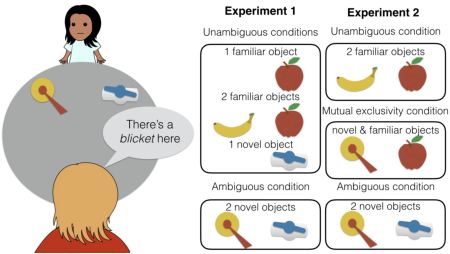
\includegraphics{figs/design-1} 

}

\caption[Study design for experiments 1 and 2]{Study design for experiments 1 and 2.}\label{fig:design}
\end{figure}
\end{CodeChunk}

\section{Experiment 1}\label{experiment-1}

In Experiment 1, we examined whether children would visually reference a
speaker more often when the speaker produced a referentially ambiguous
label compared to an unambiguous label. Children sat across from an
experimenter who labeled an object on the table between them (Figure
\ref{fig:design}). The experimenter then asked the child to place the
named object in a bucket. Across trials, there were either one or two
objects on the table, which were either familiar or novel to the child.
This design allowed us to test whether merely having more than one
object present is sufficient to increase social referencing (which could
not be ruled out by Vaish et al.), or if referential ambiguity (and thus
epistemic uncertainty) is the underlying factor. If the latter is true,
we expected children to increase their looking to the experimenter only
on trials with two unfamiliar objects, when the object-label mapping was
not known and could not be inferred.

We were interested in the amount of social referencing children
exhibited across the trial. We considered four different phases of each
trial based on the notion that children might expect different social
information at different stages of the task. Specifically, we predicted
that children might expect the speaker's gaze direction to be
informative during the labeling itself, as speakers tend to look at
objects they refer to. We predicted that later in the trial, as children
reached for an object and placed it in the bucket, they might expect
evaluative feedback about their choice (e.g., facial expressions of
encouragement or discouragement).

\subsection{Methods}\label{methods}

\subsubsection{Participants}\label{participants}

We recruited a planned sample of 80 children ages 2-5 years from the
Children's Discovery Museum in San Jose, California.\footnote{Planned
  sample size, exclusion criteria, and analysis plan preregistered at
  \url{https://osf.io/y7mvt}.} The sample included 20 2-year-olds (mean
age 32.0 months), 20 3-year-olds (mean age 42.7 months), 20 4-year-olds
(mean age 55.8 months), and 20 5-year-olds (mean age 65.2 months). An
additional 20 children participated but were removed from analyses
because they heard English less than 75\% of the time at home (\emph{n}
= 10), because they were unable to complete at least half of the trials
in the task (\emph{n} = 4), because of parental interference (\emph{n} =
1), or due to experimenter or technical errors (\emph{n} = 5).

\subsubsection{Stimuli and Design}\label{stimuli-and-design}

Children were presented with one or two objects, heard a label, and were
asked to put the labeled object in a bucket. Half of the objects were
selected to be familiar to children (e.g., a cow) and half were selected
to be novel (e.g., a nozzle). There were four possible trial types based
on the number and familiarity of the objects present: one familiar
object (F), one novel object (N), two familiar objects (FF), and two
novel objects (NN). There were three trials of each type, for a total of
twelve trials. Trial types were presented sequentially in an order that
was counterbalanced across participants. The assignment of individual
objects to trial types was counterbalanced. On F/FF trials, the familiar
label for the target object was used (e.g., ``cow''). On N/NN trials, a
novel label was used (e.g., ``dawnoo'').

The critical manipulation was of referential ambiguity; F and FF trials
were referentially unambiguous, as children were expected to be certain
about the objects and their labels. Similarly, on N trials, children
were expected to be certain about the label referent as there was only
one option. However, NN trials were referentially ambiguous, as the
novel label could apply to either novel object.

Throughout the task, the experimenter never gazed at the object they
were labeling, or responded to children's verbal or non-verbal bids for
help by indicating the correct object. Thus, children were expected to
remain uncertain about the referent throughout the trial when two novel
objects were present.

\subsubsection{Procedure}\label{procedure}

Throughout the study, the child sat at one end of a large circular
table, and the experimenter stood at the opposite end. Each trial of the
task proceeded as follows: the experimenter placed one or two objects on
the left and/or right sides of the table, out of reach of the child so
that the child could not interact with the toys during the labeling
event. For one-object trials, the location of the object (left or right)
alternated between trials.

After placing the objects, the experimenter said ``Hey look, there's a
(target) here.'' The experimenter gazed at the center of the table
rather than the object they labeled. The experimenter waited
approximately two seconds based on a visual metronome placed within view
before saying, ``Can you put the (target) in the bucket?'' They then
pushed the object(s) forward within reach of the child, and placed a
plastic bucket in the center of the table, also within reach of the
child. Prior to the twelve experimental trials, there were two training
trials: a F trial and a FF trial, to acquaint the child with the
procedure. A camera placed to the side of the experimenter captured the
participant's face, so that looking behavior could be coded from video.

\subsubsection{Coding procedure and analytic
plan}\label{coding-procedure-and-analytic-plan}

Videos were coded using DataVyu software (\url{http://datavyu.org}). For
each participant, we coded the \emph{number of times} they referenced
the experimenter throughout each trial. An alternative analytic option
would be to simply code \emph{whether or not} children looked at the
experimenter. However, during piloting, we found that most children
looked up to the experimenter at least once while they were labeling the
object, suggesting that a binary measure of looking would not be
meaningful.

Because we were interested in the precise circumstances in which
children feel uncertain enough to reference a speaker, we coded the
number of looks that occurred during four distinct phases of the trial:
a \emph{label} phase, which began at the utterance of the label and
ended when the experimenter began to slide the objects, a \emph{slide}
phase, in which the experimenter slid the object(s) into the child's
reach, a \emph{planning} phase, which began at the end of the slide and
ended when the child touched an object, and a \emph{response} phase,
which began when the child touched an object and ended when the child
released the object into the bucket. A second coder independently scored
the number of looks for one third of the trials for each participant to
establish reliability. Inter-rater reliability for the number of looks
in each phase was high, intraclass correlation \emph{r} = .97,
\emph{p}\textless{}.001.

Table \ref{tab:phases} displays the average durations of each of the
four phases. The \emph{label} and \emph{response} phases are longer on
average than the \emph{planning} and \emph{slide} phases. However, note
that we are interested in comparing the amount of social referencing
across ambiguity conditions and not across phases directly.

To quantify the effects of the number and familiarity of objects on
children's looking, along with any developmental trends, we planned to
fit a linear mixed-effects regression, beginning with the following
structure and trimming according to standard laboratory
procedures\footnote{Standard laboratory analytic procedures available at
  \url{https://osf.io/zqzsu/wiki/home/}}:
\texttt{number\ of\ looks\ \textasciitilde{}\ number\ of\ objects\ *\ familiarity\ *\ phase\ *\ age\ in\ months\ +\ (number\ of\ objects\ *\ familiarity\ \textbar{}\ subject)}.
This model specification was preregistered, as noted above.

\subsection{Results and Discussion}\label{results-and-discussion}

\subsubsection{Accuracy}\label{accuracy}

\begin{CodeChunk}
\begin{figure*}[b]

{\centering 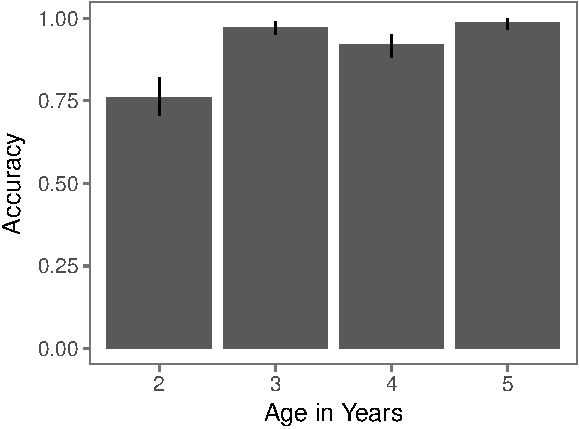
\includegraphics{figs/acc_e1-1} 

}

\caption[Accuracy for FF trials in Experiment 1]{Accuracy for FF trials in Experiment 1. Error bars are 95 percent confidence intervals.}\label{fig:acc_e1}
\end{figure*}
\end{CodeChunk}

\begin{table}[b]
\centering
\begin{tabular}{rllrr}
  \hline
 & Experiment & Phase & Mean Duration & SD \\ 
  \hline
1 & 1 & label & 5072.84 & 899.16 \\ 
  2 & 1 & slide & 872.43 & 196.83 \\ 
  3 & 1 & planning & 1253.85 & 2215.56 \\ 
  4 & 1 & response & 3646.40 & 4510.01 \\ 
   \hline
5 & 2 & label & 5239.23 & 748.05 \\ 
  6 & 2 & slide & 818.95 & 1307.27 \\ 
  7 & 2 & planning & 790.88 & 10327.45 \\ 
  8 & 2 & response & 4084.56 & 5032.37 \\ 
   \hline
\end{tabular}
\caption{Phase Durations} 
\label{tab:phases}
\end{table}

We examined children's accuracy for those trials in which a correct
response was possible (i.e., FF trials). Children sometimes put two
items in the bucket (20.0\% of trials), despite instructions to choose
only one. If they put the correct item in the bucket first followed by
the incorrect object, we counted their response as correct. If they put
the incorrect object in first, we counted their response as incorrect.
Children also occasionally declined to choose an item (0.8\% of trials);
these trials are excluded from accuracy analyses. Children's accuracy is
displayed in Table \ref{tab:acc_table}. Overall children generally chose
the correct item for FFiliar trials, indicating that they understood the
task and were motivated to answer correctly. While 3- to 5-year-olds
performed close to ceiling (92\% - 99\%), 2-year-olds were less accurate
(76\%), but still performed significantly above chance (\emph{t}(19) =
23.0 , \emph{p} \textless{}.001).

\begin{CodeChunk}
\begin{figure*}[b]

{\centering 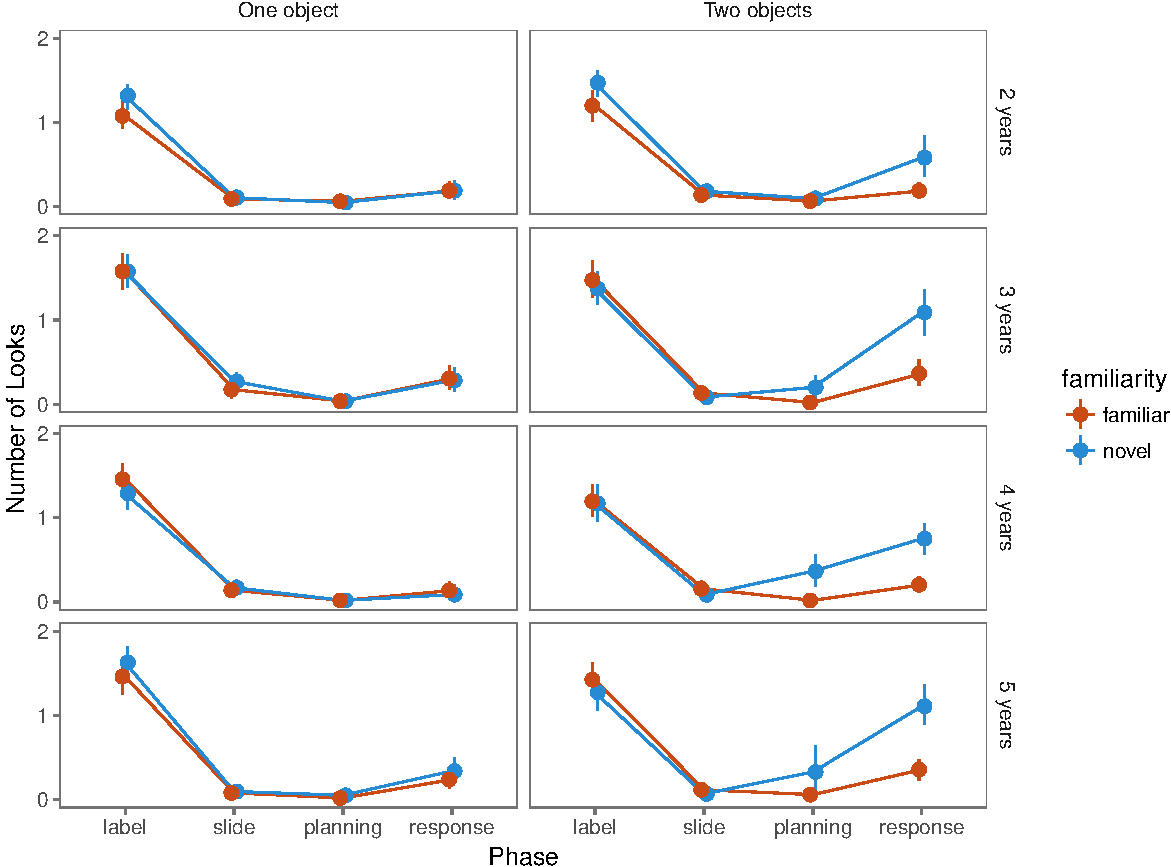
\includegraphics[width=5.75in,height=4.35in]{figs/results_e1-1} 

}

\caption[Results of Experiment 1]{Results of Experiment 1. Number of looks to the experimenter based on phase, the number and familiarity of objects present, and age. Age in months was entered as a continuous variable in regression models but is presented here as a categorical variable for visual simplicity. Error bars are 95 percent confidence intervals.}\label{fig:results_e1}
\end{figure*}
\end{CodeChunk}

\begin{table}[tb]
\centering
\begin{tabular}{lrrrrl}
 Predictor & Estimate & Std. Error & $t$ value & $p$ value &  \\ 
  \hline
Intercept & 1.38 & 0.06 & 22.58 & $<$ .001 & *** \\ 
  Num objects (2) & -0.06 & 0.06 & -1.02 & 0.31 &  \\ 
  Familiarity (N) & 0.07 & 0.06 & 1.16 & 0.25 &  \\ 
  Age & 0.01 & 0.00 & 1.85 & 0.07 & . \\ 
  Num objects (2) * Familiarity (N) & -0.06 & 0.09 & -0.74 & 0.46 &  \\ 
  Num objects (2) * Age & -0.01 & 0.00 & -1.18 & 0.24 &  \\ 
  Familiarity (N) * Age & -0.01 & 0.00 & -1.17 & 0.24 &  \\ 
  Num objects (2) * Familiarity (N) * Age & -0.00 & 0.01 & -0.57 & 0.57 &  \\ 
   \hline
\end{tabular}
\caption{Predictor estimates with standard errors and significance information for a linear mixed-effects model predicting social referencing in the label phase in Experiment 1.} 
\label{tab:exp1_l_reg}
\end{table}

\begin{table}[tb]
\centering
\begin{tabular}{lrrrrl}
 Predictor & Estimate & Std. Error & $t$ value & $p$ value &  \\ 
  \hline
Intercept & 0.12 & 0.02 & 5.06 & $<$ .001 & *** \\ 
  Num objects (2) & 0.02 & 0.03 & 0.55 & 0.58 &  \\ 
  Familiarity (N) & 0.04 & 0.03 & 1.38 & 0.17 &  \\ 
  Age & -0.00 & 0.00 & -0.44 & 0.66 &  \\ 
  Num objects (2) * Familiarity (N) & -0.07 & 0.04 & -1.69 & 0.09 & . \\ 
  Num objects (2) * Age & 0.00 & 0.00 & 0.20 & 0.84 &  \\ 
  Familiarity (N) * Age & -0.00 & 0.00 & -0.18 & 0.86 &  \\ 
  Num objects (2) * Familiarity (N) * Age & -0.00 & 0.00 & -0.84 & 0.4 &  \\ 
   \hline
\end{tabular}
\caption{Predictor estimates with standard errors and significance information for a linear mixed-effects model predicting social referencing in the slide phase in Experiment 1.} 
\label{tab:exp1_s_reg}
\end{table}

\begin{table}[tb]
\centering
\begin{tabular}{lrrrrl}
 Predictor & Estimate & Std. Error & $t$ value & $p$ value &  \\ 
  \hline
Intercept & 0.03 & 0.02 & 1.48 & 0.14 &  \\ 
  Num objects (2) & 0.01 & 0.04 & 0.26 & 0.8 &  \\ 
  Familiarity (N) & 0.00 & 0.03 & 0.12 & 0.9 &  \\ 
  Age & -0.00 & 0.00 & -0.92 & 0.36 &  \\ 
  Num objects (2) * Familiarity (N) & 0.20 & 0.05 & 4.34 & $<$ .001 & *** \\ 
  Num objects (2) * Age & 0.00 & 0.00 & 0.54 & 0.59 &  \\ 
  Familiarity (N) * Age & 0.00 & 0.00 & 0.73 & 0.47 &  \\ 
  Num objects (2) * Familiarity (N) * Age & 0.00 & 0.00 & 1.42 & 0.16 &  \\ 
   \hline
\end{tabular}
\caption{Predictor estimates with standard errors and significance information for a linear mixed-effects model predicting social referencing in the planning phase in Experiment 1.} 
\label{tab:exp1_p_reg}
\end{table}

\begin{table}[tb]
\centering
\begin{tabular}{lrrrrl}
 Predictor & Estimate & Std. Error & $t$ value & $p$ value &  \\ 
  \hline
Intercept & 0.22 & 0.04 & 5.35 & $<$ .001 & *** \\ 
  Num objects (2) & 0.05 & 0.06 & 0.96 & 0.34 &  \\ 
  Familiarity (N) & 0.01 & 0.05 & 0.18 & 0.86 &  \\ 
  Age & -0.00 & 0.00 & -0.20 & 0.84 &  \\ 
  Num objects (2) * Familiarity (N) & 0.60 & 0.07 & 8.21 & $<$ .001 & *** \\ 
  Num objects (2) * Age & 0.00 & 0.00 & 0.85 & 0.4 &  \\ 
  Familiarity (N) * Age & 0.00 & 0.00 & 0.55 & 0.58 &  \\ 
  Num objects (2) * Familiarity (N) * Age & 0.01 & 0.01 & 1.34 & 0.18 &  \\ 
   \hline
\end{tabular}
\caption{Predictor estimates with standard errors and significance information for a linear mixed-effects model predicting social referencing in the response phase in Experiment 1.} 
\label{tab:exp1_r_reg}
\end{table}

\subsubsection{Social referencing}\label{social-referencing}

Results of Experiment 1 are presented in Figure \ref{fig:results_e1}. To
test our prediction that referential ambiguity (i.e., having two novel
objects) would produce more social referencing, we fit mixed-effects
linear regression models separately for each phase with the following
structure:
\texttt{number\ of\ looks\ \textasciitilde{}\ number\ of\ objects\ *\ familiarity\ *\ age\ in\ months\ +\ (number\ of\ objects\ +\ familiarity\ \textbar{}\ subject)}.
A single model with phase as a factor did not converge, and the model
was subsequently trimmed according to our standard laboratory analytic
procedures.

We did not find any main or interaction effects of number of objects,
familiarity, or age on number of looks during the \emph{label} or
\emph{slide} phases. Thus, mere novelty or the presence of multiple
objects was not enough to increase social referencing. However, we found
an interaction effect of number of objects and familiarity during the
\emph{planning} (\(\beta\) = 0.2, \emph{p} \textless{} .001) and
\emph{response} phases (\(\beta\) = 0.6, \emph{p} \textless{} .001),
such that NN trials were associated with more looking.

There was no interaction with age in any phase.\footnote{\url{https://github.com/emilyfae/socref_uncert}}
Since an age trend in the \emph{planning} phase was apparent in the plot
(Figure \ref{fig:results_e1}), we conducted a post-hoc mixed-effects
linear regression with age group (2- and 3-year-olds vs.~4- and
5-year-olds) predicting the number of looks in the \emph{planning}
phase:
\texttt{number\ of\ looks\ \textasciitilde{}\ number\ of\ objects\ *\ familiarity\ *\ age\ group\ +\ (number\ of\ objects\ +\ familiarity\ \textbar{}\ subject)}.
We found a significant interaction of number of objects and familiarity
(\(\beta\) = 0.3, \emph{p} \textless{} .001), and a significant 3-way
interaction between number of objects, familiarity, and age group, such
that younger children looked at the experimenter less than older
children for NN trials. Although this was a post-hoc analysis, it
suggests that there may be a trend for children to respond more quickly
to uncertainty as they grow older. This could mean that they detect
uncertainty more quickly, or that they are more proactive in seeking
disambiguating information prior to initiating a response.

\begin{CodeChunk}
\begin{figure*}[b]

{\centering 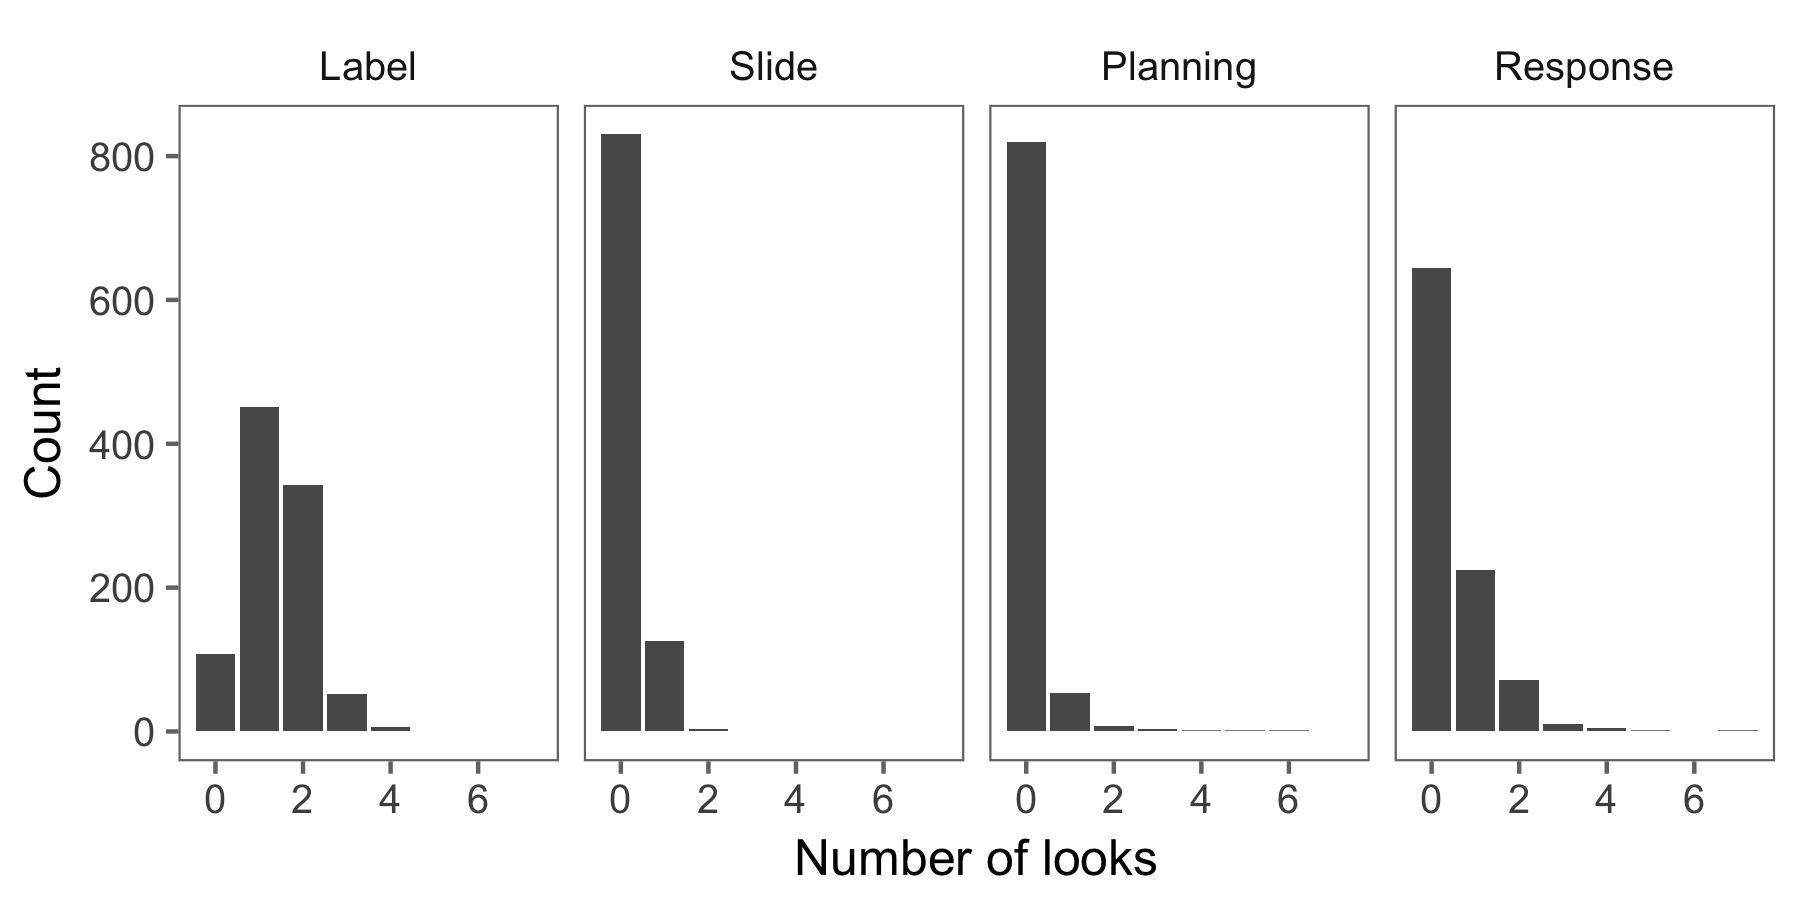
\includegraphics{figs/hist_e1-1} 

}

\caption[Distribution of the number of looks to the experimenter in each phase]{Distribution of the number of looks to the experimenter in each phase.}\label{fig:hist_e1}
\end{figure*}
\end{CodeChunk}

As discussed previously, an alternative analytic approach would be to
fit a logistic mixed-effects regression predicting \emph{whether or not}
children look to the experimenter in each phase, rather than the number
of times they do so. In support of this approach, the distribution of
looks is not normal for the slide, planning, and response phases, with
the majority of trials containing no looks to the experimenter (Figure
\textbackslash{}ref\{fig:hist\_e1). To address this issue, we
additionally fit separate logistic mixed-effects regressions with the
following structure:
\texttt{look\ (yes\ or\ no)\ \textasciitilde{}\ number\ of\ objects\ *\ familiarity\ *\ age\ group\ +\ (number\ of\ objects\ +\ familiarity\ \textbar{}\ subject)}.
A single model with phase as a factor did not converge.

The results of these analyses were similar to those of the linear
models; number of objects and familiarity interacted in the
\emph{planning} and \emph{response} phases such that there was more
likely to be a look when there were two novel objects, (\(\beta\)s =
1.4202815, 1.9757203, \emph{p}s \textless{}.05 \& \textless{}.001.

In summary, children looked to the experimenter more often when planning
and executing a response under uncertainty. These results suggest that
children were aware that they did not have sufficient knowledge to
answer independently, and referenced the speaker to resolve this
uncertainty.{]}xz

Notably, and in contrast to Vaish et al., we did not find the expected
effect of referential ambiguity in the \emph{label} phase. It is
possible that children failed to predict that they would need more
information until later in the trial, when they were actually faced with
making a decision. Another possibility is that children's looking was at
ceiling during the labeling phase, perhaps because children tend to look
at someone who is speaking regardless of the need for referential
disambiguation. A third possibility is that this finding is an artifact
of our design, in which the experimenter gazed at the center of the
table rather than the referent of the label. Children may have realized
that the experimenter's gaze direction during labeling was not
informative. Alternatively, children may have found it strange to
interact with an experimenter who did not gaze at the object they were
labeling, which may have produced unnatural patterns of social
referencing. Experiment 2 tests these possibilities and examines whether
children's social referencing is sensitive to graded uncertainty.

\section{Experiment 2}\label{experiment-2}

Experiment 2 was designed to replicate Experiment 1 and investigate
whether children's social referencing is sensitive to uncertainty based
on graded evidence about a label's referent. A hallmark of successful
uncertainty monitoring is being less confident when the probability of
accuracy is lower (Kiani \& Shadlen, 2009). This ability includes
awareness of complete ignorance, but also of graded evidence in mental
representations (Fleming, Dolan, \& Frith, 2012; Ghetti, Lyons,
Lazzarin, \& Cornoldi, 2008), which may be important for predicting
outcomes and guiding behavior.

To examine children's social referencing on the basis of graded
referential evidence, we added 1-novel-1-familiar trials. For these
trials, we expected that children would be able to infer the referent by
excluding the familiar object as a possibility. For example, when a toy
lion and a novel item were present, they could exclude that the speaker
was referring to the lion as a ``blicket'' (Markman \& Wachtel, 1988).
Since we did not observe any difference between F and N trials, we
eliminated single-object trials, leaving the FF and NN trials. We
predicted that children might be less certain about their choice on
these trials compared to when the label and referent were familiar to
them (FF trials), but more confident than when there are no cues to
reference (NN trials).

To further manipulate the availability of referential evidence, we
varied between participants whether or not the experimenter's gaze
during labeling was informative (they gazed at either the referent of
their label or the center of the table). This manipulation also allowed
us to determine whether children selectively reference gaze during
labeling when gaze is informative. For Experiment 2, we restricted the
sample to 3- and 4-year-olds, as there was no effect of age in our
preregistered analyses, but a trend for younger children to engage in
selective referencing earlier in the trial than older children.

\subsection{Methods}\label{methods-1}

\subsubsection{Participants}\label{participants-1}

We recruited a planned sample of 80 children ages 3-4 years from the
Children's Discovery Museum in San Jose, California.\footnote{Planned
  sample size, exclusion criteria, and analysis plan (including model
  specification) preregistered at \url{https://osf.io/y7mvt/}.} The
sample included 40 3-year-olds (mean age 42.9 months) and 40 4-year-olds
(mean age 53.5 months). An additional 20 children participated but were
removed from analyses because they heard English less than 75\% of the
time at home (\emph{n} = 9), because they were unable to complete at
least half of the trials in the task (\emph{n} = 7), or due to
experimenter or technical errors (\emph{n} = 4).

\subsubsection{Stimuli and Design}\label{stimuli-and-design-1}

The stimuli and design were similar to Experiment 1 but included three
trial types: FF, NN, and FN. There were four of each trial type,
totaling twelve trials. In addition, we manipulated the experimenter's
gaze behavior between participants. For half of the participants, the
experimenter looked at the center of the table while labeling objects;
for the remaining half, they looked directly at the objects they
labeled.

\subsubsection{Procedure}\label{procedure-1}

The experimental and coding procedures were identical to Experiment 1,
except that there were three practice trials (two familiar trials and
one novel trial). We chose this approach so that children could
experience both familiar and novel stimuli during practice, but would
not be discouraged by an overly difficult practice session. Inter-rater
reliability for the number of looks in each phase was again high,
intraclass correlation \emph{r} = .97, \emph{p}\textless{}.001.

The mean durations of the phases for Experiment 2 are presented in Table
\ref{tab:phases}. They varied in length as in Experiment 1. Children's
accuracy for trials with a correct answer (i.e., FF, FN, and all trials
with gaze) was calculated using the same criteria as in Experiment 1
(Table \ref {tab:acc_table}).

\subsection{Results and Discussion}\label{results-and-discussion-1}

\subsubsection{Accuracy}\label{accuracy-1}

\begin{CodeChunk}
\begin{figure*}[b]

{\centering 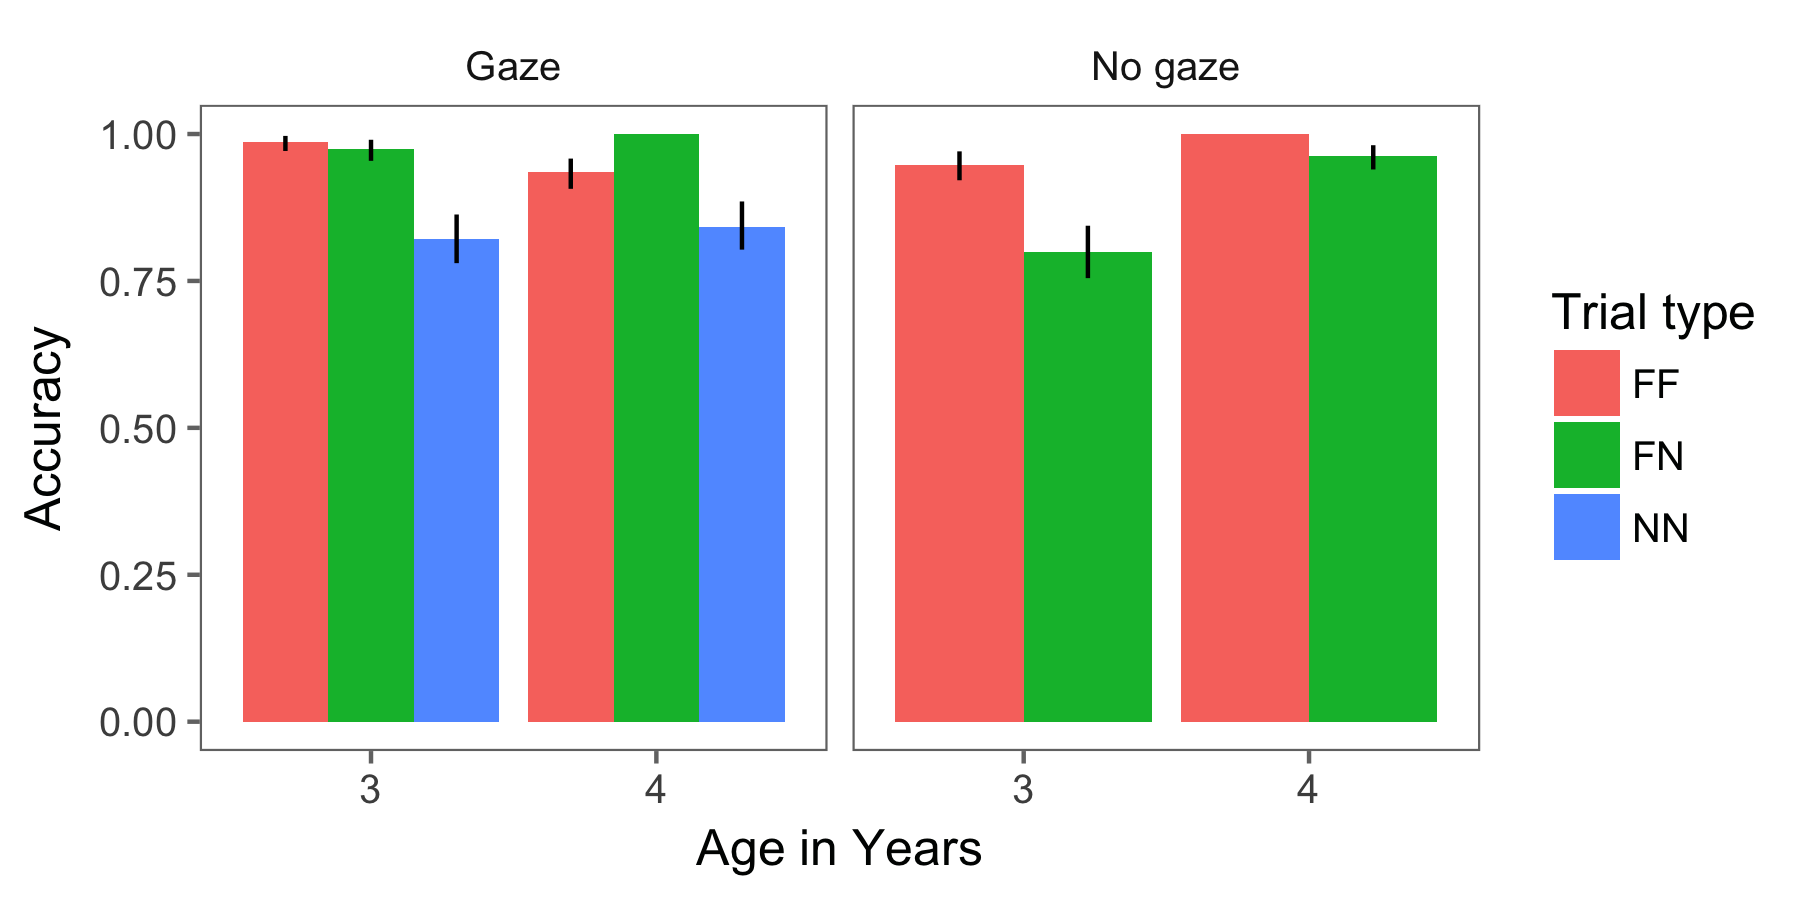
\includegraphics{figs/acc_e2-1} 

}

\caption[Accuracy for trials with a correct answer available (FF and FN, and all gaze trials) in Experiment 2]{Accuracy for trials with a correct answer available (FF and FN, and all gaze trials) in Experiment 2. Error bars are 95 percent confidence intervals.}\label{fig:acc_e2}
\end{figure*}
\end{CodeChunk}

To quantify the effects of familiarity, gaze, and age on accuracy, we
fit the following mixed-effects logistic regression model:
\texttt{correct\ \textasciitilde{}\ trial\ type\ *\ gaze\ +\ age\ in\ months\ +\ (1\textbar{}\ subject)}.
Accuracy was significantly lower for novel (\(\beta\) = -2.3, \emph{p}
\textless{} .001) and mutual trials (\(\beta\) = -2.2, \emph{p}
\textless{} .001) compared to familiar trials, and trial type interacted
with gaze condition such that accuracy was significantly higher in the
gaze condition for novel (\(\beta\) = 3.4, \emph{p} \textless{} .001)
and mutual trials (\(\beta\) = 1.1, \emph{p} \textless{} .001). Age did
not significantly predict accuracy (\(\beta\) = 0.2, \emph{p} = .12).

\subsubsection{Social referencing and referential
ambiguity}\label{social-referencing-and-referential-ambiguity}

Children's social referencing based on trial type and gaze condition are
presented in Figure \ref{fig:results_e2}. To quantify the main and
interactive effects of familiarity, gaze informativity, phase, and age
on social referencing, we fit a mixed-effects linear regression model
with the following structure:
\texttt{number\ of\ looks\ \textasciitilde{}\ familiarity\ *\ age\ in\ months\ *\ gaze\ *\ phase\ +\ (familiarity\ \textbar{}\ subject)}.
In contrast to Experiment 1, a model with phase as a predictor
converged.

First, do children reference a speaker more often when the objects and
label are novel? Phase interacted with familiarity such that the
\emph{response} phase of novel trials was associated with significantly
more looks (\(\beta\) = 0.3, \emph{p} \textless{} .001). This result is
consistent with results from Experiment 1. However, in contrast to
Experiment 1, the number of looks was not significantly greater for
novel trials in the \emph{planning} phase.

We were also interested in whether mutual exclusivity trials would
elicit an intermediate amount of uncertainty. We observed a three-way
interaction of familiarity, gaze, and phase, such that the response
phase of mutual exclusivity trials in the no-referential-gaze condition
was associated with significantly more looks (\(\beta\) = -0.2, \emph{p}
\textless{} .01). Thus, mutual exclusivity trials were associated with
greater looking only when the experimenter did not provide informative
gaze. This finding is intriguing given that children should be able to
solve mutual exclusivity trials without gaze information. Instead, these
results suggest that children relatively uncertain while making a
decision if excluding the familiar object is their only cue to
reference, but this uncertainty is resolved if the speaker's gaze is
informative. On the other hand, informative gaze during labeling did not
lessen social referencing for novel trials, suggesting that gaze
information alone was not sufficient to reduce uncertainty. Instead,
both gaze information and mutual exclusivity provided evidence about a
label-object pairing, and children required both types of evidence to
feel certain about their response.

Finally, we observed a four-way interaction such that the
\emph{response} phase of novel trials in the gaze condition was
associated with more looking with increasing age (\(\beta\) = 0.0,
\emph{p} \textless{} .01), suggesting that children may become more
selective in their social referencing as they get older. It may be that
children improve in their ability to monitor the need for disambiguating
information, or they may become more likely to recognize that social
information can be a source of disambiguation.

We did not observe selective social referencing during the \emph{label}
phase, even when referential gaze was available. This result rules out
the possibility that children are less selective during labeling because
they learned that gaze direction was not informative.

\begin{CodeChunk}
\begin{figure*}[b]

{\centering 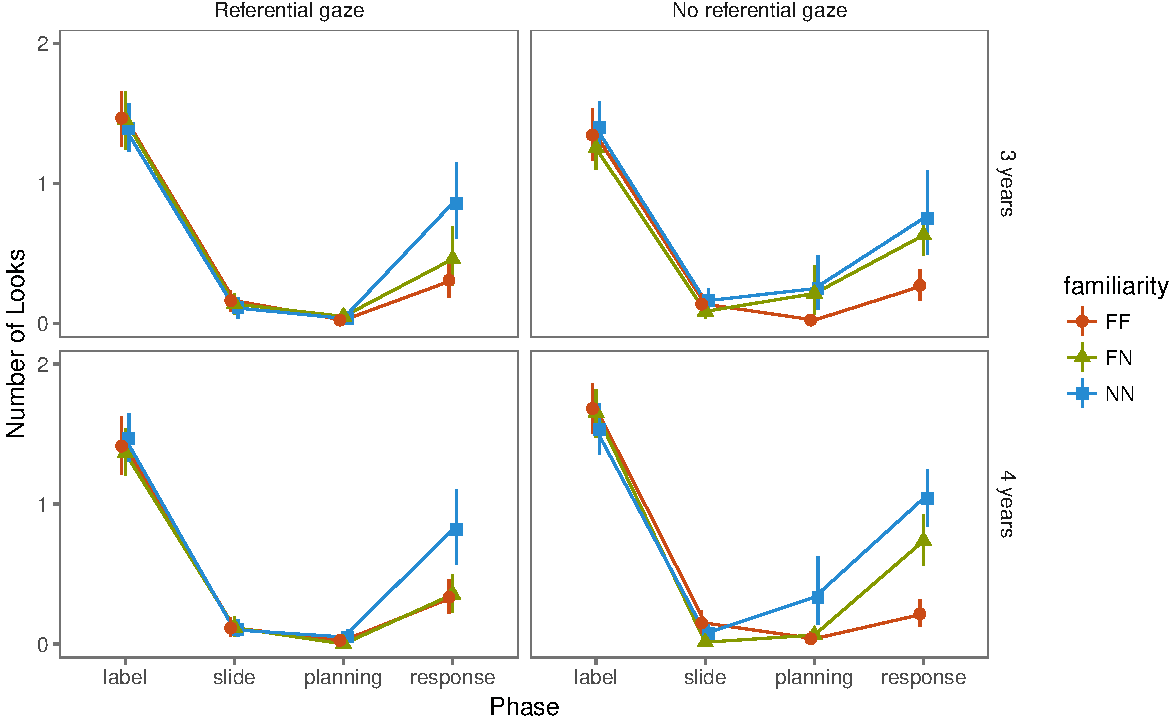
\includegraphics[width=5.75in,height=3.5in]{figs/results_e2-1} 

}

\caption[Results of Experiment 2]{Results of Experiment 2. Number of looks to the experimenter based on phase, trial type, gaze condition, and age. Age in months was entered as a continuous variable in regression models but is presented here as a categorical variable for visual simplicity. Error bars are 95 percent confidence intervals.}\label{fig:results_e2}
\end{figure*}
\end{CodeChunk}

\begin{table}[tb]
\centering
\begin{tabular}{lrrrrl}
 Predictor & Estimate & Std. Error & $t$ value & $p$ value &  \\ 
  \hline
Intercept & 0.14 & 0.06 & 2.62 & 0.01 & ** \\ 
  Trial type(FN) & -0.09 & 0.07 & -1.27 & 0.21 &  \\ 
  Trial type(NN) & -0.02 & 0.08 & -0.29 & 0.77 &  \\ 
  Age & 0.00 & 0.01 & 0.27 & 0.79 &  \\ 
  Gaze(Y) & -0.01 & 0.08 & -0.09 & 0.93 &  \\ 
  Phase(Label) & 1.36 & 0.07 & 18.71 & $<$ .001 & *** \\ 
  Phase(Planning) & -0.11 & 0.07 & -1.54 & 0.12 &  \\ 
  Phase(Response) & 0.10 & 0.07 & 1.38 & 0.17 &  \\ 
  Trial type(FN) * Age & -0.01 & 0.01 & -0.80 & 0.43 &  \\ 
  Trial type(NN) * Age & -0.01 & 0.01 & -0.66 & 0.51 &  \\ 
  Trial type(FN) * Gaze & 0.08 & 0.10 & 0.77 & 0.44 &  \\ 
  Trial type(NN) * Gaze & -0.01 & 0.11 & -0.10 & 0.92 &  \\ 
  Age * Gaze & -0.00 & 0.01 & -0.35 & 0.72 &  \\ 
  Trial type(FN) * Phase(Label) & 0.02 & 0.10 & 0.24 & 0.81 &  \\ 
  Trial type(NN) * Phase(Label) & -0.02 & 0.10 & -0.23 & 0.82 &  \\ 
  Trial type(FN) * Phase(Planning) & 0.21 & 0.10 & 2.01 & 0.04 & * \\ 
  Trial type(NN) * Phase(Planning) & 0.28 & 0.10 & 2.77 & 0.01 & ** \\ 
  Trial type(FN) * Phase(Response) & 0.53 & 0.10 & 5.09 & $<$ .001 & *** \\ 
  Trial type(NN) * Phase(Response) & 0.68 & 0.10 & 6.52 & $<$ .001 & *** \\ 
  Age * Phase(Label) & 0.02 & 0.01 & 2.07 & 0.04 & * \\ 
  Age * Phase(Planning) & -0.00 & 0.01 & -0.31 & 0.76 &  \\ 
  Age * Phase(Response) & -0.00 & 0.01 & -0.09 & 0.93 &  \\ 
  Gaze * Phase(Label) & -0.06 & 0.10 & -0.59 & 0.56 &  \\ 
  Gaze * Phase(Planning) & -0.00 & 0.10 & -0.00 & 1 &  \\ 
  Gaze * Phase(Response) & 0.08 & 0.10 & 0.79 & 0.43 &  \\ 
  Trial type(FN) * Age * Gaze & 0.01 & 0.02 & 0.46 & 0.65 &  \\ 
  Trial type(NN) * Age * Gaze & 0.01 & 0.02 & 0.49 & 0.62 &  \\ 
  Trial type(FN) * Age * Phase(Label) & 0.01 & 0.02 & 0.73 & 0.47 &  \\ 
  Trial type(NN) * Age * Phase(Label) & -0.00 & 0.02 & -0.19 & 0.85 &  \\ 
  Trial type(FN) * Age * Phase(Planning) & -0.00 & 0.02 & -0.04 & 0.96 &  \\ 
  Trial type(NN) * Age * Phase(Planning) & 0.01 & 0.02 & 0.78 & 0.43 &  \\ 
  Trial type(FN) * Age * Phase(Response) & 0.02 & 0.02 & 1.14 & 0.25 &  \\ 
  Trial type(NN) * Age * Phase(Response) & 0.02 & 0.02 & 1.37 & 0.17 &  \\ 
  Trial type(FN) * Gaze * Phase(Label) & -0.05 & 0.15 & -0.32 & 0.75 &  \\ 
  Trial type(NN) * Gaze * Phase(Label) & 0.05 & 0.15 & 0.32 & 0.75 &  \\ 
  Trial type(FN) * Gaze * Phase(Planning) & -0.20 & 0.15 & -1.35 & 0.18 &  \\ 
  Trial type(NN) * Gaze * Phase(Planning) & -0.23 & 0.15 & -1.61 & 0.11 &  \\ 
  Trial type(FN) * Gaze * Phase(Response) & -0.43 & 0.15 & -2.97 & 0 & ** \\ 
  Trial type(NN) * Gaze * Phase(Response) & -0.14 & 0.15 & -0.96 & 0.34 &  \\ 
  Age * Gaze * Phase(Label) & -0.02 & 0.02 & -1.14 & 0.26 &  \\ 
  Age * Gaze * Phase(Planning) & 0.01 & 0.02 & 0.45 & 0.65 &  \\ 
  Age * Gaze * Phase(Response) & -0.00 & 0.02 & -0.18 & 0.86 &  \\ 
  Trial type(FN) * Age * Gaze * Phase(Label) & -0.01 & 0.02 & -0.41 & 0.68 &  \\ 
  Trial type(NN) * Age * Gaze * Phase(Label) & 0.01 & 0.02 & 0.47 & 0.64 &  \\ 
  Trial type(FN) * Age * Gaze * Phase(Planning) & -0.00 & 0.02 & -0.07 & 0.94 &  \\ 
  Trial type(NN) * Age * Gaze * Phase(Planning) & -0.02 & 0.02 & -0.64 & 0.52 &  \\ 
  Trial type(FN) * Age * Gaze * Phase(Response) & -0.04 & 0.02 & -1.64 & 0.1 &  \\ 
  Trial type(NN) * Age * Gaze * Phase(Response) & -0.05 & 0.02 & -1.94 & 0.05 & . \\ 
   \hline
\end{tabular}
\caption{Predictor estimates with standard errors and significance information for a linear mixed-effects model predicting social referencing in Experiment 1.} 
\label{tab:exp2_reg}
\end{table}

\subsubsection{Social referencing and
accuracy}\label{social-referencing-and-accuracy}

\begin{table}[tb]
\centering
\begin{tabular}{lrrrrl}
 Predictor & Estimate & Std. Error & $t$ value & $p$ value &  \\ 
  \hline
Intercept & 0.11 & 0.09 & 1.21 & 0.23 &  \\ 
  Acc(Y) & 0.01 & 0.09 & 0.06 & 0.95 &  \\ 
  Age & -0.00 & 0.01 & -0.30 & 0.76 &  \\ 
  Phase(Label) & 0.96 & 0.12 & 8.00 & $<$ .001 & *** \\ 
  Phase(Planning) & 0.10 & 0.12 & 0.81 & 0.42 &  \\ 
  Phase(Response) & 1.31 & 0.12 & 10.91 & $<$ .001 & *** \\ 
  Acc(Y) * Age & 0.00 & 0.01 & 0.21 & 0.84 &  \\ 
  Acc(Y) * Phase(Label) & 0.41 & 0.12 & 3.31 & $<$ .001 & *** \\ 
  Acc(Y) * Phase(Planning) & -0.17 & 0.12 & -1.33 & 0.18 &  \\ 
  Acc(Y) * Phase(Response) & -0.99 & 0.12 & -7.99 & $<$ .001 & *** \\ 
  Age * Phase(Label) & 0.04 & 0.02 & 1.90 & 0.06 & . \\ 
  Age * Phase(Planning) & 0.02 & 0.02 & 0.99 & 0.32 &  \\ 
  Age * Phase(Response) & 0.02 & 0.02 & 0.98 & 0.33 &  \\ 
  Acc(Y) * Age * Phase(Label) & -0.02 & 0.02 & -1.16 & 0.25 &  \\ 
  Acc(Y) * Age * Phase(Planning) & -0.02 & 0.02 & -1.00 & 0.32 &  \\ 
  Acc(Y) * Age * Phase(Response) & -0.03 & 0.02 & -1.25 & 0.21 &  \\ 
   \hline
\end{tabular}
\caption{Predictor estimates with standard errors and significance information for a linear mixed-effects model predicting social referencing based on accuracy in Experiment 2.} 
\label{tab:exp2acc_reg}
\end{table}

In the metacognitive framework, confidence judgments are generally
compared for correct and incorrect responses, with lower confidence for
incorrect responses taken as evidence for metacognitive accuracy (refs).
Here, a parallel approach would be to examine the amount of social
referencing children demonstrate for correct and incorrect responses.

To this end, we fit a mixed-effects linear regression model with the
following structure:
\texttt{number\ of\ looks\ \textasciitilde{}\ accuracy\ *\ age\ in\ months\ *\ phase\ +\ (1\ \textbar{}\ subject)}.
The number of looks was collapsed across trial types and gaze
conditions, since there were relatively few incorrect trials overall and
none at all for some of the conditions. Results showed that accuracy and
phase interacted such that children looked at the experimenter
significantly more during the labeling phase of accurate trials
(\(\beta\) = 0.4, \emph{p} \textless{} .001), and significantly less in
the \emph{response} phase of accurate trials (\(\beta\) = -1.0, \emph{p}
\textless{} .001).

These findings confirm that children reference the experimenter more
while responding incorrectly. Importantly, this analysis was restricted
to trials in which there was a correct response available (i.e., because
the target was familiar or could be inferred by excluding the familiar
distracter or observing the speaker's gaze). Thus, children's looking is
sensitive not only to complete ignorance, but other factors that affect
accuracy, which might include graded evidence or relative familiarity
with the stimuli).

Additionally, children were more likely to answer correctly if they
referenced the speaker during the labeling phase. This pattern could be
due to children obtaining referential evidence from the experimenter's
gaze in the gaze condition, or it could represent trials in which
children were more engaged in the task.

\begin{CodeChunk}
\begin{figure*}[b]

{\centering 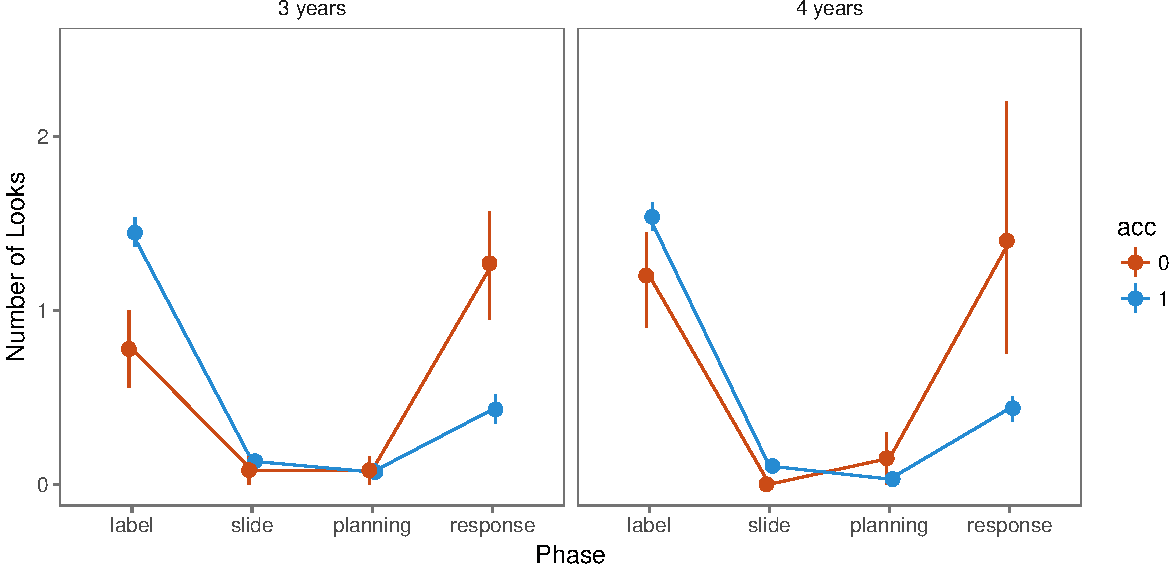
\includegraphics[width=6in,height=3in]{figs/acc_results_e2-1} 

}

\caption[Results of Experiment 2]{Results of Experiment 2. Number of looks to the experimenter based on accuracy, phase, and age, collapsed across trial types and gaze conditions. Age in months was entered as a continuous variable in regression models but is presented here as a categorical variable for visual simplicity. Error bars are 95 percent confidence intervals. }\label{fig:acc_results_e2}
\end{figure*}
\end{CodeChunk}

\section{General Discussion}\label{general-discussion}

During the preschool years, children are increasingly able to actively
gather information through help-seeking and exploration (Chouinard et
al., 2007; Schulz \& Bonawitz, 2007). Do children monitor their own
uncertainty to guide these behaviors, or are they indiscriminate with
regard to underlying knowledge states? Here, we examined whether young
children's social referencing during a word-learning task was driven by
uncertainty about a label's referent.

We found that referential ambiguity strongly predicted children's social
referencing. Specifically, we observed this selectivity when children
were forced to decide which object the speaker was referring to. We
speculate that children referenced the speaker during the decision
process because they expected evaluative feedback about their choice,
either implicitly through the adult's facial expressions, or through an
explicit response. This idea is consistent with other recent research
that has found that preschoolers and toddlers seek help selectively when
a problem is difficult or they are less skilled (Goupil et al., 2016;
Vredenburgh \& Kushnir, 2015).

Most intriguingly, we found that children's looking was driven by graded
referential evidence. This is important given that being able to monitor
the likelihood of accuracy based on graded evidence is assumed important
for decision-making and behavioral regulation later in development
(refs). In the case of mutual exclusivity trials, children could solve
the problem of reference by excluding the familiar item (Markman \&
Wachtel, 1988). Thus, unlike novel trials, they likely had some signal
about the correct object-label mapping. If children simply monitored the
presence or absence of such signals, they would have consistently
treated mutual exclusivity trials as familiar trials. Instead, their
social referencing depended on a combination of cues from mutual
exclusivity and gaze informativity, suggesting that they are sensitive
to graded evidence and seek disambiguating information only when
uncertainty is relatively high. Children's greater social referencing on
trials with only one cue to reference (i.e., mutual exclusivity trials
with no referential gaze and novel trials with referential gaze)
additionally suggests that children may remain uncertain about a new
label-object mapping if they have not received confirmation of its
accuracy, for example, through explicit feedback or gaze direction.

On the other hand, we found no evidence for selective social referencing
as the object was being labeled. One possibility is that young children
do not recognize the need for disambiguating information until they need
to make a decision. Another possibility is that preschool-aged children
spontaneously look at a speaker regardless of ambiguity, and additional
looking was not needed or possible. Notably, Vaish et al. observed
selective referencing during labeling among infants. Since infants in
that study were holding one of the objects during labeling, referencing
the speaker would have required them to disengage from that object, and
may therefore have been more costly, promoting selectivity. Future
research with preschoolers that includes a greater trade-off between
attentional options would help to distinguish among these possibilities.

Overall, these results provide evidence that preschool-aged children
monitor graded uncertainty in their mental representations and act on
that uncertainty through spontaneous information-seeking.

\section{Acknowledgements}\label{acknowledgements}

We thank Veronica Cristiano for assisting with data collection. EH was
supported by a generous gift from Kinedu SAPI de CV.

\section{References}\label{references}

\setlength{\parindent}{-0.1in} \setlength{\leftskip}{0.125in} \noindent

\hypertarget{refs}{}
\hypertarget{ref-Balcomb2008}{}
Balcomb, F. K., \& Gerken, L. (2008). Three-year-old children can access
their own memory to guide responses on a visual matching task.
\emph{Developmental Science}, \emph{11}(5), 750--760.

\hypertarget{ref-Baldwin1991}{}
Baldwin, D. A. (1991). Infants' contribution to the achievement of joint
reference. \emph{Child Development}, \emph{62}(5), 875--890.

\hypertarget{ref-Call2001}{}
Call, J., \& Carpenter, M. (2001). Do apes and children know what they
have seen? \emph{Animal Cognition}, \emph{3}(4), 207--220.

\hypertarget{ref-Chouinard2007}{}
Chouinard, M. M., Harris, P. L., \& Maratsos, M. P. (2007). Children's
questions: A mechanism for cognitive development. \emph{Monographs of
the Society for Research in Child Development}, \emph{72}, 1--129.

\hypertarget{ref-Corriveau2009}{}
Corriveau, K., \& Harris, P. L. (2009). Preschoolers continue to trust a
more accurate informant 1 week after exposure to accuracy information.
\emph{Developmental Science}, \emph{12}(1), 188--193.

\hypertarget{ref-Coughlin2014}{}
Coughlin, C., Hembacher, E., Lyons, K. E., \& Ghetti, S. (2014).
Introspection on uncertainty and judicious help-seeking during the
preschool years. \emph{Developmental Science}, \emph{18}(6), 957--971.

\hypertarget{ref-Csibra2006}{}
Csibra, G., \& Gergely, G. (2006). Social learning and social cognition:
The case for pedagogy. In Y. Munakata \& M. H. Johnson (Eds.),
\emph{Processes of change in brain and cognitive development} (pp.
249--274). Oxford: Oxford University Press: Oxford University Press.

\hypertarget{ref-Flavell1995}{}
Flavell, J. H., Green, F. L., Flavell, E. R., Harris, P. L., \&
Astington, J. W. (1995). Young children's knowledge about thinking.
\emph{Monographs of the Society for Research in Child Development},
i--iii--v--vi--1--113.

\hypertarget{ref-Fleming2012}{}
Fleming, S. M., Dolan, R. J., \& Frith, C. D. (2012). Metacognition:
computation, biology and function. \emph{Philosophical Transactions of
the Royal Society B: Biological Sciences}, \emph{367}(1594), 1280--1286.

\hypertarget{ref-Ghetti2008}{}
Ghetti, S., Lyons, K. E., Lazzarin, F., \& Cornoldi, C. (2008). The
development of metamemory monitoring during retrieval: The case of
memory strength and memory absence. \emph{Journal of Experimental Child
Psychology}, \emph{99}(3), 157--181.

\hypertarget{ref-Goupil2016}{}
Goupil, L., Romand-Monnier, M., \& Kouider, S. (2016). Infants ask for
help when they know they dont know. \emph{Proceedings of the National
Academy of Sciences}, \emph{113}(13), 3492--3496.

\hypertarget{ref-Hembacher2014}{}
Hembacher, E., \& Ghetti, S. (2014). Dont look at my answer: Subjective
uncertainty underlies preschoolers exclusion of their least accurate
memories. \emph{Psychological Science}, \emph{25}(9),
0956797614542273--1776.

\hypertarget{ref-Ho2017}{}
Ho, M. K., MacGlashan, J., Littman, M. L., \& Cushman, F. (2017). Social
is special: A normative framework for teaching with and learning from
evaluative feedback. \emph{Cognition}, 1--16.

\hypertarget{ref-Johnson1991}{}
Johnson, M. H., Dziurawiec, S., Ellis, H., \& Morton, J. (1991).
Newborns preferential tracking of face-like stimuli and its subsequent
decline. \emph{Cognition}, \emph{40}, 1--19.

\hypertarget{ref-Kiani2009}{}
Kiani, R., \& Shadlen, M. N. (2009). Representation of Confidence
Associated with a Decision by Neurons in the Parietal Cortex.
\emph{Science}, \emph{324}, 759--764.

\hypertarget{ref-Koenig2009}{}
Koenig, M. A., Clement, F., \& Harris, P. L. (2009). Trust in testimony:
Children's use of true and false statements. \emph{Psychological
Science}, \emph{15}, 694--698.

\hypertarget{ref-Li2014}{}
Li, Q.-G., Heyman, G. D., Xu, F., \& Lee, K. (2014). Young children's
use of honesty as a basis for selective trust. \emph{Journal of
Experimental Child Psychology}, \emph{117}(C), 59--72.

\hypertarget{ref-Lyons2011a}{}
Lyons, K. E., \& Ghetti, S. (2011). The development of uncertainty
monitoring in early childhood. \emph{Child Development}, \emph{82}(6),
1778--1787.

\hypertarget{ref-Markman1988}{}
Markman, E. M., \& Wachtel, G. F. (1988). Children's use of mutual
exclusivity to constrain the meanings of words. \emph{Cognitive
Psychology}, \emph{20}, 121--157.

\hypertarget{ref-Ruggeri2017}{}
Ruggeri, A., Sim, Z. L., \& Xu, F. (2017). ``Why is Toma late to school
again?'' Preschoolers identify the most informative questions.
\emph{Developmental Science}.

\hypertarget{ref-Sabbagh2001}{}
Sabbagh, M. A., \& Baldwin, D. A. (2001). Learning words from
knowledgeable versus ignorant speakers: Links between preschoolers
theory of mind and semantic development. \emph{Child Development},
\emph{72}, 1054--1070.

\hypertarget{ref-Schulz2007}{}
Schulz, L. E., \& Bonawitz, E. B. (2007). Serious fun: Preschoolers
engage in more exploratory play when evidence is confounded.
\emph{Developmental Psychology}, \emph{43}(4), 1045--1050.

\hypertarget{ref-Shafto2012}{}
Shafto, P., Goodman, N. D., \& Frank, M. C. (2012). Learning from
others: The consequences of psychological reasoning for human learning.
\emph{Perspectives on Psychological Science}, \emph{7}(4), 341--351.

\hypertarget{ref-Sim2017}{}
Sim, Z. L., \& Xu, F. (2017). Learning higher-order generalizations
through free play: Evidence from two- and three-year-old children.
\emph{Developmental Psychology}.

\hypertarget{ref-Sobel2013}{}
Sobel, D. M., \& Kushnir, T. (2013). Knowledge matters: How children
evaluate the reliability of testimony as a process of rational
inference. \emph{Psychological Review}, \emph{120}, 779=797.

\hypertarget{ref-Sodian2012}{}
Sodian, B., Thoermer, C., Kristen, S., \& Perst, H. (2012).
Metacognition in infants and young children. In M. J. Beran, J. Brandl,
J. Perner, \& J. Proust (Eds.), \emph{Foundations of metacognition} (pp.
119--133).

\hypertarget{ref-Sorce1985}{}
Sorce, J. F., Emde, R. N., Campos, J., \& Klinnert, M. D. (1985).
Maternal emotional signaling: Its effect on the visual cliff behavior of
1-year-olds. \emph{Developmental Psychology}, \emph{21}, 195--200.

\hypertarget{ref-Stahl2015}{}
Stahl, A. E., \& Feigenson, L. (2015). Observing the unexpected enhances
infants learning and exploration. \emph{Science}, \emph{348}(6230),
91--94.

\hypertarget{ref-Striano2000}{}
Striano, T., \& Rochat, P. (2000). Emergence of selective social
referencing in infancy. \emph{Infancy}, \emph{1}, 253--264.

\hypertarget{ref-Vaish2011}{}
Vaish, A., Demir, Ö. E., \& Baldwin, D. (2011). Thirteen- and
18-month-old infants recognize when they need referential information.
\emph{Social Development}, \emph{20}(3), 431--449.

\hypertarget{ref-Vredenburgh2015}{}
Vredenburgh, C., \& Kushnir, T. (2015). Young children's help-seeking as
active information gathering. \emph{Cognitive Science}, \emph{40}(3),
697--722.

\hypertarget{ref-Walden1988}{}
Walden, T. A., \& Ogan, T. A. (1988). The development of social
referencing. \emph{Child Development}, \emph{59}(5), 1230--1240.

\hypertarget{ref-Yurovsky2015}{}
Yurovsky, D., \& Frank, M. C. (2015). An integrative account of
constraints on cross-situational learning. \emph{Cognition},
\emph{145}(C), 53--62.

\hypertarget{ref-Zarbatany1985}{}
Zarbatany, L., \& Lamb, M. E. (1985). Social referencing as a function
of information source: Mothers versus strangers. \emph{Infant Behavior
and Development}, \emph{8}, 25--33.

\bibliography{}

\end{document}
